\documentclass[border=0mm]{standalone}

\usepackage{contour}
\usepackage{ifthen}
\usepackage{tcolorbox}
\usepackage{tikz}
\usepackage{xcolor}

%%%%%%%%%%%%%%%%%%%%%%%%%%%%%%%%%%%%%%%%%%%%%%%%%%%%%%%%%%%%%%%%%%%%%%%%%%%%%
% File: colours.tex
% Author: Edmund Mulligan <edmund@edmundmulligan.name>
% Version: 1.0
% This file is part of the workbook for Non-Violent Communication.
% Description: Contains the definitions of the colours used in the workbook.
%%%%%%%%%%%%%%%%%%%%%%%%%%%%%%%%%%%%%%%%%%%%%%%%%%%%%%%%%%%%%%%%%%%%%%%%%%%%%
\definecolor{tem_cyan}{rgb}{.2, .8, .8}
\definecolor{tem_purple}{rgb}{0.706, 0.051, 0.831}
\definecolor{tem_grey}{RGB}{245, 245, 245}

 \definecolor{tem_blue1}{RGB}{240,248,255} % AliceBlue
 \definecolor{tem_blue2}{RGB}{135,206,250} % LightSkyBlue
 \definecolor{tem_blue3}{RGB}{100,149,237} % CornflowerBlue
 \definecolor{tem_blue4}{RGB}{0,0,255}     % Blue
 \definecolor{tem_blue5}{RGB}{0,0,128}     % Navy


\begin{document}
  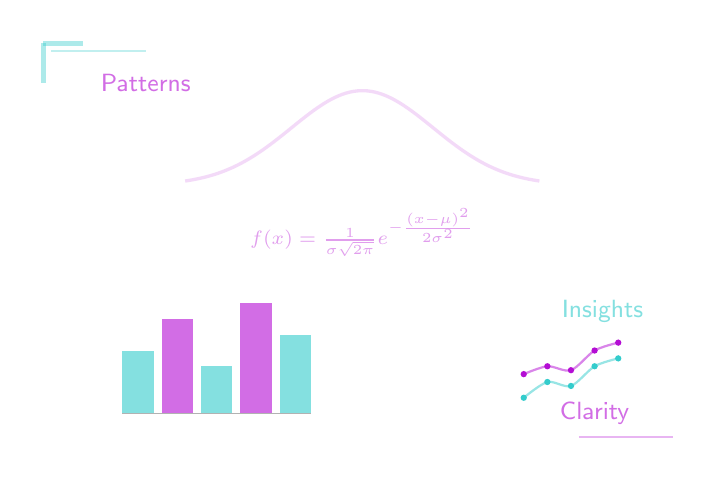
\begin{tikzpicture}
    % Business card dimensions: 85mm x 55mm (approx 8.5cm x 5.5cm)
    % Define the card background
    \fill[white] (0,0) rectangle (8.5,5.5);
    
    % Bell curve (normal distribution) in background - iconic and recognizable
    \begin{scope}[transparency group, opacity=0.15]
      \draw[tem_purple, very thick, smooth, samples=100, domain=-2.5:2.5] 
        plot ({4.25 + 0.9*\x}, {3.5 + 1.2*exp(-\x*\x/2)});
    \end{scope}
    
    % Simple bar chart visualization (clean and accessible)
    \begin{scope}[shift={(1.2,0.6)}]
      \fill[tem_cyan, opacity=0.6] (0,0) rectangle (0.4,0.8);
      \fill[tem_purple, opacity=0.6] (0.5,0) rectangle (0.9,1.2);
      \fill[tem_cyan, opacity=0.6] (1.0,0) rectangle (1.4,0.6);
      \fill[tem_purple, opacity=0.6] (1.5,0) rectangle (1.9,1.4);
      \fill[tem_cyan, opacity=0.6] (2.0,0) rectangle (2.4,1.0);
      % Base line
      \draw[black, opacity=0.3] (0,0) -- (2.4,0);
    \end{scope}
    
    % Clean line graph (moved to avoid bell curve)
    \begin{scope}[shift={(6.3,0.8)}]
      \draw[tem_cyan, thick, opacity=0.5] 
        plot[smooth] coordinates {(0,0) (0.3,0.2) (0.6,0.15) (0.9,0.4) (1.2,0.5)};
      \draw[tem_purple, thick, opacity=0.5] 
        plot[smooth] coordinates {(0,0.3) (0.3,0.4) (0.6,0.35) (0.9,0.6) (1.2,0.7)};
      % Data points
      \foreach \x/\y in {0/0, 0.3/0.2, 0.6/0.15, 0.9/0.4, 1.2/0.5} {
        \fill[tem_cyan] (\x,\y) circle (0.04);
      }
      \foreach \x/\y in {0/0.3, 0.3/0.4, 0.6/0.35, 0.9/0.6, 1.2/0.7} {
        \fill[tem_purple] (\x,\y) circle (0.04);
      }
    \end{scope}
    
    % Normal distribution PDF formula (closer to bell curve)
    \node[tem_purple, font=\scriptsize, opacity=0.4, align=center] at (4.25, 2.9) 
      {$f(x) = \frac{1}{\sigma\sqrt{2\pi}} e^{-\frac{(x-\mu)^2}{2\sigma^2}}$};
    
    % Simple friendly labels (no complex notation)
    \node[tem_purple, font=\small\sffamily, opacity=0.6] at (1.5, 4.8) {Patterns};
    \node[tem_cyan, font=\small\sffamily, opacity=0.6] at (7.3, 1.9) {Insights};
    \node[tem_purple, font=\small\sffamily, opacity=0.6] at (7.2, 0.6) {Clarity};
    
    % Subtle decorative elements suggesting data flow
    \draw[tem_cyan, thick, opacity=0.3] (0.3,5.2) -- (1.5,5.2);
    \draw[tem_purple, thick, opacity=0.3] (7.0,0.3) -- (8.2,0.3);
    
    % Small corner accent
    \draw[tem_cyan, line width=2pt, opacity=0.4] (0.2,5.3) -- (0.2,4.8);
    \draw[tem_cyan, line width=2pt, opacity=0.4] (0.2,5.3) -- (0.7,5.3);
    
  \end{tikzpicture}
\end{document}
